\documentclass{article}
\usepackage[english]{babel}
\usepackage[utf8]{inputenc}
\usepackage{amsmath}
\usepackage{graphicx}
\usepackage[colorinlistoftodos]{todonotes}

\title{CIS 519 Problem Set 1}

\author{Gabrielle Merritt}

\date{\today}

\begin{document}
\maketitle
\part{Problem Set}
\section{Decision Tree Learning}
\subsection{Information Gain} 
At root node for a decision tree in this domain, what are the information gains associated with the Outlook and Humidity attributes? (Use a threshold of 75 for humidity). Be sure to show computations.

\paragraph{Solution:}
Entropy $S$ of the root node can be represented as:
$$S = -(\frac{5}{14}\log_2{\frac{5}{14}})- (\frac{9}{14}\log_2{\frac{9}{14}}) = .940 $$

For Humidity the weighted average entropy of the children $\leq 75 and >75$  
$$\bar{S_h} = \frac{5}{14}[-(\frac{1}{5}\log_2{\frac{1}{5}})- (\frac{4}{5}\log_2{\frac{4}{5}})] + \frac{9}{14}[-(\frac{4}{9}\log_2{\frac{4}{9}})- (\frac{5}{9}\log_2{\frac{5}{9}})]= .541
$$
For Outlook the average entropy of children Sunny,Overcast, and Rain 
$$\bar{S_o} = \frac{5}{14}[-(\frac{3}{5}\log_2{\frac{3}{5}})- (\frac{2}{5}\log_2{\frac{2}{5}})] + \frac{4}{14}[-(\frac{0}{4}\log_2{\frac{0}{4}})- (\frac{4}{4}\log_2{\frac{4}{4}})] + \frac{5}{14}[-(\frac{2}{5}\log_2{\frac{2}{5}})- (\frac{3}{5}\log_2{\frac{3}{5}})] = .6936
$$

Information gain $I$ can be computed as 
$$I_g = S - \bar{S_c}
$$
Therefore Information gain for Humidity ($I_h$) and Outlook($I_o$) are:

$$I_h = S - \bar{S}_h = .399
$$
$$I_o = S -\bar{S}_o =.246$$

\subsection{Gain Ratios}
Again at the root node, what are the gain ratios associated with the Outlook and Humidity
attributes (using the same threshold as in (a))? 
Be sure to show your computations.
\paragraph{Solution:}
Gain Ratio ($GainRatio(S,A)$) is defined as
$$ GainRatio(S,A) = \frac{Gain(S,A)}{SplitInfo(S,A)}
$$ 

$$ GainRatio(S,Humidity) = \frac{I_h}{-\frac{5}{14}\log_2\frac{5}{14} - \frac{9}{14}\log_2\frac{9}{14}} = .424
$$

$$ GainRatio(S,Outlook) = \frac{I_o}{-\frac{5}{14}\log_2\frac{5}{14} - \frac{4}{14}\log_2\frac{4}{14} - \frac{5}{14}\log_2\frac{5}{14}} = .156
$$

\subsection {Decision Tree} 
Draw the complete (unpruned) decision tree, showing the class predictions at the leaves. 
\linebreak
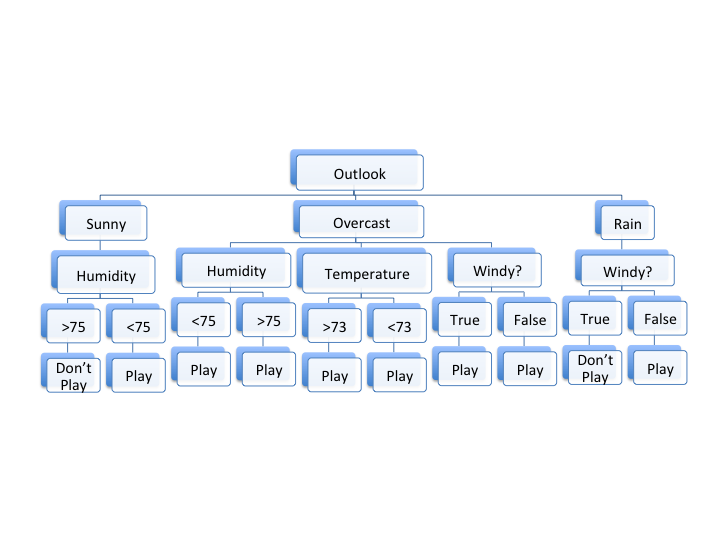
\includegraphics[width = \linewidth]{dTree_un.png}
\linebreak

\section{Linear Regression and kNN}

Suppose we have a sample of n pairs $(x_i; y_i)$ drawn i.i.d. from the following
distribution:
\newline
$x_i\in X$,the set of instances
\newline 
$y_i = f(x_i) + \epsilon_i$,where $f()$ is the regression function
\newline 
$\epsilon_i \sim G(0,\sigma^2)$,a Gaussian with mean 0 and variance 2
\newline 
We can construct an estimator for $f()$ that is linear in the $y_i$,

$$f(x_0) =\displaystyle\sum\limits_{i=1}^n l_i(x_0; X)y_i
$$

where the weights $l_i(x_0;X)$ do not depend on the $y_i$, but do depend on the entire training set $X$. Show that
both linear regression and k-nearest neighbour regression are members of this class of estimators. 
\newline 
Explicitly describe the weights $l_i(x_0;X)$ for each of these algorithms.

\paragraph {Solution:}
k-NN can be represented as the equation 
$$f(x_0) = \frac{1}{K} \displaystyle\sum\limits_{i =1}^K y_i
$$
Which we can deduce that $l_i (x_0; X)  = 1/K$ which k depends on the number of nearest neighbours 
\newline
For general closed form solution for linear regression
\newline  
 $ f(X) = X\theta  $  where $ \theta = (X^TX)^{-1}XY $
 $$f(X_0) =[\begin{matrix} 1 & x_0 \end{matrix} ][(X^TX)^{-1}XY]$$ 
 So we can say that 
 $$l_i(X_0;X) = [\begin{matrix} 1 & x_0 \end{matrix} ] (X^TX)^{-1}X $$ 
 Which shows that the weight $l_i(x_0;X)$ is not dependent on $y_i$ 
 
 \section{Decision Trees and Linear Discriminants}
 Describe in detail how to modify a classic decision tree algorithm (ID3 / C4.5) to obtain oblique splits (i.e,
splits that are not parallel to an axis).
In order to obtain oblique splits for a decision tree algorithm such as ID3, or C4.5 instead of creating a parallel axis split on a single real valued attribute. Oblique splits are obtained by a linear combination of real valued attributes. 
Source: Kohavi, Ron, and Ross Quinlan. Decision Tree Discovery.  10 Oct. 1999. http://ai.stanford.edu/~ronnyk/treesHB.pdf

\part{Programming Exercises Analysis}
\section {Linear Regression} 
\section {Logistic Regression}
For my varied values of lambda I noticed that the larger lambda became the faster $||\theta -\theta_old||^{2}_2 \leq \epsilon$, and in cases for large lambdas ,the worse the classifier worked, and hte longer it took to run 
\linebreak
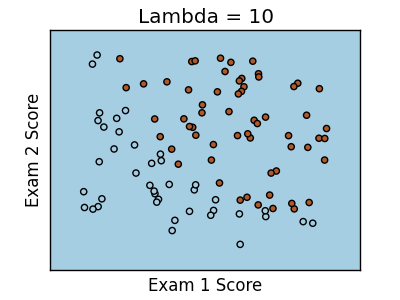
\includegraphics[width = \linewidth]{Lambda10.png}

\paragraph{}
For small values of lambda the slower the gradient decent, without much gain  
\linebreak
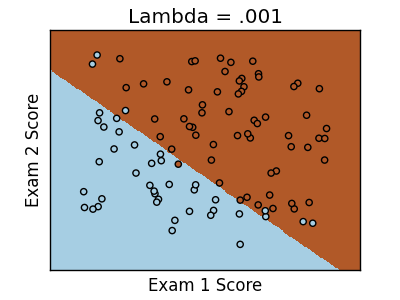
\includegraphics[width = \linewidth]{Lambda_001.png}
\linebreak
the figure above is for $ \lambda = .001$ 
\paragraph{}
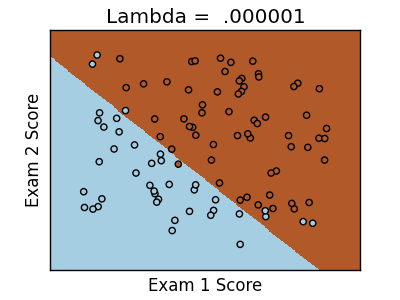
\includegraphics[width = \linewidth]{Lambda_000001.png}
the figure above is for $ \lambda = .000001$ 
\paragraph{}
\section{Non linear Decision Surface}
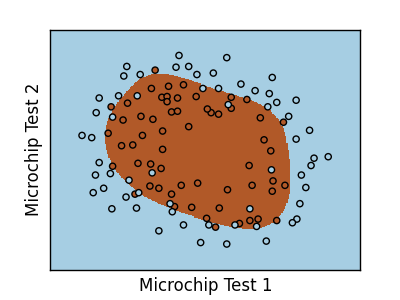
\includegraphics[width = \linewidth]{NLDS.png}
\section{Learning Curve}
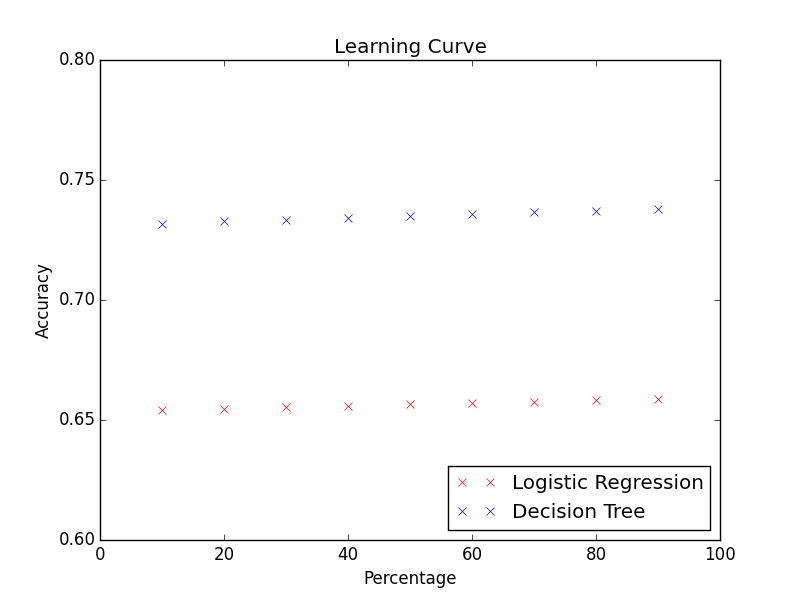
\includegraphics[width =\linewidth]{learningcurve.png}

\end{document}
